\section{Compute Link Budget}\label{sec:link_budget}

\subsection{Line-Of-Sight Propagation}\label{subsec:los_propagation}
At low frequency (below approximately 3 MHz) radio signals travel as ground waves, which follow the Earth's curvature due to diffraction with the layers of the atmosphere.
However, at higher frequencies and in lower levels of the atmosphere, neither of these effects are significant. Thus any obstruction between the transmitting antenna (transmitter) and the receiving antenna (receiver) will block the signal, just like the light that the eye may sense. Therefore, since the ability to visually see a transmitting antenna (disregarding the limitations of the eye's resolution) roughly corresponds to the ability to receive a radio signal from it, the propagation characteristic of VHF and higher radio frequency (>30 MHz) paths is called line-of-sight. The farthest possible point of propagation is referred to as the radio horizon.

The radio horizon is the locus of points at which direct rays from an antenna are tangential to the surface of the Earth. If the Earth were a perfect sphere and there were no atmosphere, the radio horizon would be a circle.
This way the greatest distance at which a receiver can see the transmitter is explained in the following paragraph.

First, we are going to derive a general expression and after that apply it to a scenario with a UAV and a GS. In figure  \ref{fig:GeometricDist_general} the relationship between the height of the observer above sea level (O point) and the distance d which is between it and the horizon (H point) is shown. Finding this distance is done by the use of the pythagorean theorem. With some simple mathematical calculations the distance d is derived in the following:

\begin{equation}\label{eq:los_distToHorizon}
	(R+h)^2 = R^2+d^2\nonumber \\
	\Rightarrow R^2+2hR+h^2 = R^2+d^2 \Rightarrow d^2 = 2hR + h^2 \\
	\Rightarrow d = \sqrt{2hR + h^2}
\end{equation} 

\begin{figure}
    \hfill
    \subfigure[Geometrical distance to the horizon]{
    	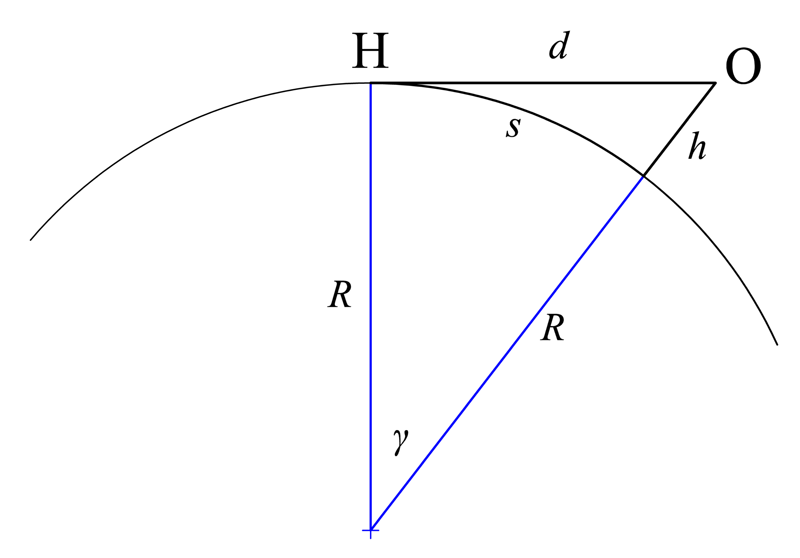
\includegraphics[scale=4]{figures/GeometricDistanceToHorizonOneTriangle.png} 
		\label{fig:GeometricDist_general}}
	\hfill
    \subfigure[Geometrical distance from UAV to GS]{
    	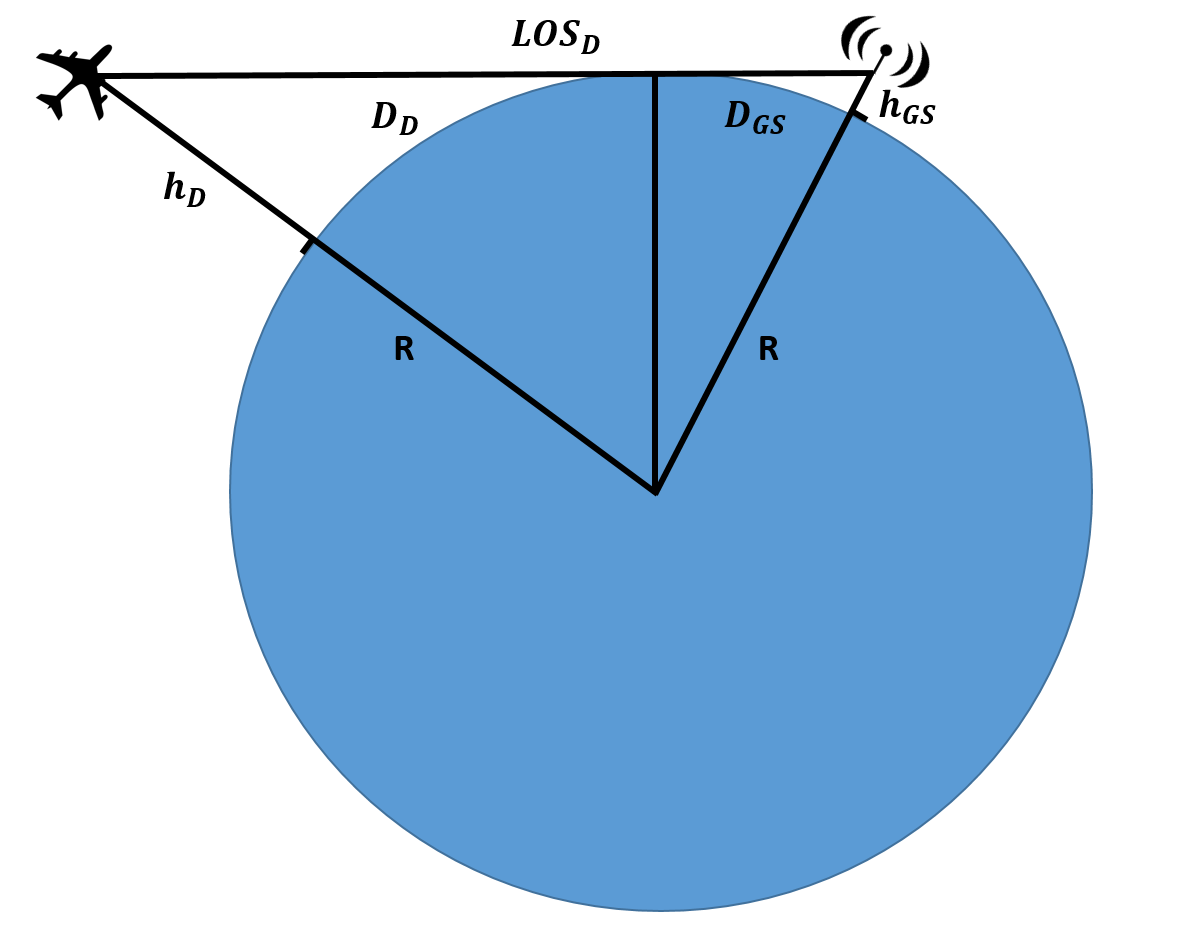
\includegraphics[scale=0.3]{figures/GeometricDistanceToHorizonTwoTriangle.png} 
    	\label{fig:GeometricDist_droneBasestation}}
    \hfill
    \caption{Geometrical distance to the horizon, Pythahorean theorem}
\end{figure}

On figure \ref{fig:GeometricDist_droneBasestation} it is shown that the two objects are a GS and an UAV. Both of them won't be higher then approx 100 meter and since R is radius of the Earth, $2hR$ >> $h^2$ and $h^2$ is therefore neglected in equation \ref{eq:los_distToHorizon}. The two distances $D_D$ and $D_B$ have the same expressions in both cases:
\begin{align*}
	D_D [km] &= \sqrt{2\cdot R \cdot h_D + h_{D}^2} \approx \sqrt{2\cdot 6.378\cdot h_D} = \sqrt{12.756\cdot h_D} = 3.57\cdot \sqrt{h_D} \\
	D_B [km] &= \sqrt{2\cdot R \cdot h_B + h_{B}^2} \approx \sqrt{2\cdot 6.378\cdot h_B} = \sqrt{12.756\cdot h_B} = 3.57\cdot \sqrt{h_B}
\end{align*}

To calculate the distance $D_{DB}$:
\begin{align}
	D_{DB}[km]	 &= D_D + D_B \approx 3.57\cdot \sqrt{h_D} + 3.57\cdot \sqrt{h_B} = {3.57\cdot (\sqrt{h_D} + \sqrt{h_B}} )
\end{align}

\subsection{LOS Distance Example}
Lets take an example where the aircraft is at $h_D = 100m$ and the ground station at $h_B = 20m$. The distance between them is as follows:
\begin{equation*}
	D_{DB}[km] = 3.57\cdot (\sqrt{100} + \sqrt{20}) = 51.67km
\end{equation*}

\subsection{Free Space Path Loss}\label{subsec:path_loss}
\paragraph{}
The free space path loss (FSPL) is the loss in signal strength that occurs when an electromagnetic wave travels over a line of sight path in free space. In these circumstances there are no obstacles that might cause the signal to be reflected, refracted, or that might cause additional attenuation. Equation \ref{eq:path_losses} represents the loss in signal strength in dB.

\begin{equation}\label{eq:path_losses}
	L_{FS} = 20\lg\left (\frac{4\pi \cdot d}{\lambda} \right)
\end{equation}

The wave length can also be described by a relationship between the frequency and the velocity of light. This relationship is described by the equation \ref{eq:vel_freq_wavelen1}.

\begin{equation}\label{eq:vel_freq_wavelen1}
	\lambda = \frac{c}{f}
\end{equation}

Explanation of the parameters.
\begin{itemize}
	\item d - distance from transmitter to receiver [m]
	\item $\lambda$ - wavelength of the signal [m]
	\item c - speed of light constant $3\cdot 10^8$ [m/s] 
	\item f - frequency of signal [Hz]
\end{itemize}

Considering our problem we will look into the worst case scenario, which would be the maximum distance between GS and UAV. 
\begin{equation*}
	Assume 
	\begin{cases}
	d_{max} = \sqrt{x^2+y^2}\\
	\text{f} = f\text{GHz (Should be permitted by law})\\
	\end{cases}
\end{equation*}

Computing signal wavelength:
\begin{equation}\label{eq:vel_freq_wavelen2}
	\lambda = \frac{c}{f} 
	        = \frac{3\cdot 10^{8}}{f\cdot 10^{9}}
	        = \frac{3}{10f}m
\end{equation}

Computing path loss:
\begin{align*}\label{eq:path_loses_calc}
	L = 20\lg\left (\frac{4\pi d}{\lambda} \right) dB 
	 &= 20\lg\left (\frac{4\pi \sqrt{x^2+y^2}}{\frac{3}{10f}} \right) dB\\ 
	 &= 20\lg\left (\frac{4\pi \sqrt{x^2+y^2}\cdot 10f}{ 3} \right) dB
\end{align*}
\noindent \textbf{As an observation, higher distance value between GS and UAV will result in higher path loss.}

\subsection{Link Budget}\label{subsec:link_budget}
\paragraph{}
A link budget is accounting of all of the gains and losses from the transmitter, through the medium  to the receiver in a telecommunication system. It accounts for the attenuation of the transmitted signal due to propagation, as well as the antenna gains, feedline and miscellaneous losses. 
\begin{equation*}\label{eq:link_budget} 
 		\text{Received Power (dBm)} = \text{Transmitted Power (dBm)} + \text{Gains (dB)} - \text{Losses(dB)}
\end{equation*}

In more detailed a common radio link looks like this:

\begin{equation*}\label{eq:link_budget} 
 		P_{RX} = P_{TX} + G_{TX} - L_{TX} - L_{FS} - L_{M} + G_{RX} - L_{RX}
\end{equation*}

Note that decibels are logarithmic measurements, so adding decibels is equivalent to multiplying the actual numeric ratios.